\section{Balls-in-bins batching}

As we will see in the next section, applying Monte Carlo accounting to correlated noise mechanisms requires time linear in the number of possible participation patterns. For $n$-round DP-SGD with Poisson sampling, this is $2^n$. Shuffling reduces the number of possible participation patterns, and is generally considered a more practical variant, but is hard to do privacy analysis for because the participations of different examples are not independent like in Poisson sampling.

To alleviate the issues with both Poisson sampling and shuffling, we propose \textit{balls-in-bins batching}. Informally, balls-in-bins batching forms batches using the balls-in-bins process, where examples are balls and batches are bins:

\begin{definition}
In \textbf{balls-in-bins batching}, we form batches as follows. Let $b$ be the number of batches per epoch we wish to use and let $E$ be the number of epochs that we train.
Also denote by $n=b\cdot E$ the total number of training iterations.
For each example $d$, we independently include it in exactly one of $B_1, B_2, \ldots, B_b$ uniformly at random. We then iterate through the batches in round robin fashion, i.e. in iteration $i$ of our learning algorithm we use batch $B_{i \pmod b}$ (abusing notation to let e.g. $2b \pmod b = b$).
\end{definition}

\begin{figure}
    \centering
    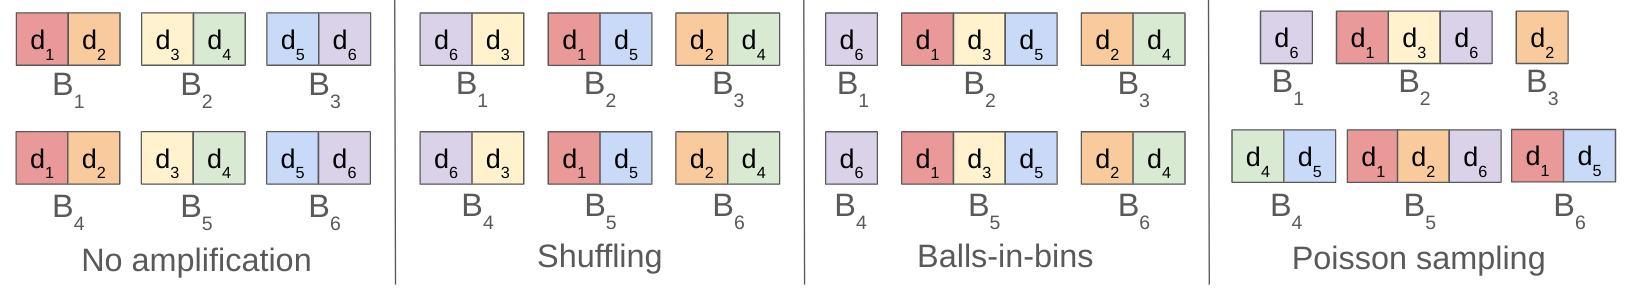
\includegraphics[width=0.95\linewidth]{other_figures/amplificationmethods.png}
    \caption{A comparison of the how different amplification methods might form batches. Here, we use $n = 6$ rounds, and form $b = 3$ batches per epoch for $E = 2$ epochs (visually represented as one row for each epoch). Note that shuffling uses fixed batch sizes, and all methods but Poisson sampling use the same batching across epochs and enforce exactly one participation per example per epoch.}
    \label{fig:amplificationmethods}
\end{figure}

In Figure~\ref{fig:amplificationmethods} we give a visualization of balls-in-bins batching and other standard methods for forming batches. The following lemma shows that the following pair of distributions is a dominating pair for the correlated noise mechanism $\bfx + \bfC^{-1} \bfz$ with balls-in-bins batching:
\begin{align*}
  P &= \frac{1}{b}\sum_{i=1}^{b} N(\bfm_i, \sigma^2 I), \text{ where } \bfm_i = \sum_{j=0}^{E-1} |\bfC|_{1:n, b\cdot j + i} \\
  Q &= N(0, \sigma^2 I),
\end{align*}
where $|\bfC|$ is the matrix whose entries are the absolute values of corresponding entry in $\bfC$.

\begin{lem}[Dimension-reduction for balls-in-bins batching]
\label{lem:bib-dim-red}
Suppose $\bfC \in \R^{n \times n}$ is a lower-triangular matrix with non-negative entries.
Then $P, Q$ (resp. $Q, P$) as defined above is a dominating pair for the correlated noise mechanism with balls-in-bins batching under the add (resp. remove) adjacency. 
\end{lem}


\begin{proof}
We will use Lemma 4.5 of \cite{choquettechoo2024privacy}, restated here for convenience:

\begin{lem}
Let $\bfc_1, \ldots, \bfc_k \in \mathbb{R}^{n \times p}$. Let $\bfc_1', \ldots, \bfc_k' \in \mathbb{R}^n$ be such that $\ltwo{\bfc_i[j, :]} \leq \bfc_i'(j)$ for all $i, j$. Then letting

\[P = N(0, \sigma^2 \mathbb{I}_{(n \times p) \times (n \times p)}), Q = \sum_i p_i N(\bfc_i, \sigma^2 \mathbb{I}_{(n \times p) \times (n \times p)}) \]    
\[P' = N(0, \sigma^2 \mathbb{I}_{n \times n}), Q' = \sum_i p_i N(\bfc_i', \sigma^2 \mathbb{I}_{n \times n}),\]

for all $\alpha$ we have $H_\alpha(P, Q) \leq H_\alpha(P', Q')$. Furthermore, this holds even if the $j$th row of each $\bfc_i$ is chosen as a function of the first $j-1$ rows of $P, Q$ (subject to $\ltwo{\bfc_i[j, :]} \leq \bfc_i'(j)$) while $\bfc_i'$ remain fixed.
\end{lem}

We give the proof for the add adjacency. Proving $P, Q$ is a dominating pair for the add adjacency implies $Q, P$ is a dominating pair for the remove adjacency by Lemma 29 of~\cite{zhu22optimal}.

Because each user is assigned to their batch independently, we can assume without loss of generality that contributions from all users other than the differing user are always $0$. In more detail, by post-processing, we can assume that we release the contributions to the input matrix of all examples except the differing user's. Let $\bfx$ be these contributions, and $\bfx'$ be $\bfx$ plus the contribution of the differing user. Then distinguishing $\bfC \bfx + \bfz$ and $\bfC \bfx' + \bfz$ is equivalent to distinguishing $\bfz$ and $\bfC (\bfx' - \bfx) + \bfz$, exactly the setting where all users except the differing user only contribute $0$.

Now, for the input matrix $\bfx \in \R^{n \times p}$, the rows have at most unit norm in the entries where the differing user participates and 0 everywhere else.
If the differing user is assigned to the $i$th batch, it is immediate by triangle inequality that
$
  \norm{(\bfC \bfx)_{k, :}}
  \leq \sum_{j=0}^{E-1}|\bfC|_{k, b\cdot j + i}
$. 
Because every user participates in each batch with probability $\frac{1}{b}$,
we can apply Lemma 4.5 of \citet{choquettechoo2024privacy} to exactly get that
the correlated noise mechanism with balls-with-bins batching is dominated by the pair $P, Q$.
\end{proof}

For simplicity of presentation, we will focus on the add adjacency in the rest of the paper. It is easy to extend results to the remove adjacency, and for the add-and-remove adjacency we can simply take the worse of the two adjacencies' privacy guarantees (paying a factor of 2 in the failure probability of \cref{thm:bernstein} by a union bound). We also remark that~\cref{lem:bib-dim-red} (and any results in our paper for the add/remove adjacency) can be readily extended to the replace adjacency using recent results of \citet{schuchardt2024unified}.

\mypar{Advantages of balls-in-bins batching} In addition to being more amenable for Monte Carlo analysis than shuffling or Poisson sampling, we believe balls-in-bins batching may be more practical than Poisson sampling for various reasons. First, one way to implement balls-in-bins batching to form $b$ batches is as follows: We sample $(c_1, c_2, \ldots, c_b)$ from the multinomial random variable with $|D|$ trials and $b$ equally likely outcomes. We shuffle the dataset once, and then we operate in multiple streaming passes over the shuffled dataset. In iteration $i$, we take the next $c_{i \pmod b}$ examples from the dataset stream.

Hence, up to the choice of variable batch size (which we will discuss how to make practical in Section~\ref{sec:practical}), balls-in-bins batching is no harder to implement than shuffling, which is generally considered to be a practical batch sampling method. As a function of requiring little overhead compared to shuffling, balls-in-bins batching avoids some of the practical issues with Poisson sampling. For example, shuffling and balls-in-bins are both memory-efficient if implemented in an offline manner as the shuffled dataset is the same size as the original dataset. In contrast, if we implement Poisson sampling in an offline manner, to store all batches formed by Poisson sampling we need to write each example $B n /|D|$ times in expectation, which can be much larger than 1. 

Shuffling and balls-in-bins are also guaranteed to give strict privacy improvements over deterministic multi-epoch training because they are sampling from a set of multi-epoch participation patterns. In contrast, as \citet{chua2024private} demonstrated, in some settings the privacy guarantees of Poisson sampling can actually be worse than deterministic batching, since Poisson sampling risks over-sampling some examples. For the same reasons, shuffling and balls-in-bins  batching are more secure in that they remain no less private than deterministic multi-epoch batching even if the randomness in the batches were somehow leaked (e.g. through a PRNG attack, or through monitoring communications during distributed training) whereas Poisson sampling can make the privacy much worse than deterministic multi-pass batching if the batches are leaked. 

\section{Monte Carlo Accounting for Correlated Noise Mechanisms}\label{sec:mcmm}

\subsection{Calibrating $\sigma$}

Now, suppose we are given a lower triangular matrix $\bfC \in \R^{n \times n}$ with non-negative entries and we aim to find the minimum noise-multiplier $\sigma$ so that the balls-in-bins mechanism is $(\eps, \delta')$-DP.
This $\delta'$ will be slightly smaller than $\delta$ so that Algorithm~\ref{alg:wrapper} is $(\epsilon, \delta)$-DP and outputs $\bot$ with very small probability.
We approach this by drawing a sample of the dominating PLD and employing a bisection root-finding algorithm on $\sigma$.

To do this, we first recall the dominating distributions,
\[ P_{\bfC,\sigma} = \frac{1}{b}\sum_{i=1}^{b} N(\bfm_i, \sigma^2 I), \text{ where } \bfm_i = \sum_{j=0}^{E-1} |\bfC|_{1:n, b\cdot j + i}, \qquad Q_{\sigma} = N(0, \sigma^2 I).\]

Hence we can sample $Y \sim PLD(P_{\bfC, \sigma}, Q_\sigma)$ by first sampling $X \sim P_{\bfC,\sigma}$ and computing $Y = \log \left(\frac{P_{\bfC,\sigma}}{Q_\sigma}(X)\right)$. Note that computing $Y$ is efficient since $P_{\bfC,\sigma}$ has only $b$ modes.
To make the sampling independent of $\sigma$, we can instead sample $i\sim Uni([b])$ and $Z \sim N(0, I)$ then for any $\sigma$ compute $Y = \log \left(\frac{P_{\bfC,\sigma}}{Q_\sigma}(\bfm_i + \sigma \cdot Z)\right)$.
This process is summarized in Algorithm~\ref{alg:sigma}, which uses the function  $\hat{\delta}$ to estimate the $\delta$ at a fixed $\sigma$.
The inner computation of $\hat{\delta}$ is easily parallelizable, as it is a simple average over a given sample size.
On top of this, a bisection algorithm is run, which can converge\footnote{To show bisection search converges, if $\sigma_{max}$ is the $\sigma$ achieving the target DP guarantee without amplification (which we easily can compute using existing accounting libraries), $\hat{\delta}(0; \ldots) = 1 > \delta$ and $\hat{\delta}(\sigma_{max}; \ldots) < \delta$ (whp). In turn, $\hat{\delta}(\sigma; \ldots) = \delta$ for some $\sigma \in [0, \sigma_{max}]$ and bisection converges to this point by continuity of $\hat{\delta}$.} to within $\Delta$ additive error in only $O(\log(1/\Delta))$ many iterations because $\sigma$ is a scalar. 

\begin{algorithm}[htb]
\caption{Finding $\sigma$} \label{alg:sigma}
 \hspace*{\algorithmicindent} \textbf{Inputs:} Target $(\epsilon, \delta)$-DP guarantee, sample size $m$, matrix $\bfC$.
\begin{algorithmic}[1]
\State $i_1\dots i_m \simiid Uni([b])$ \State $Z_1, \dots, Z_m \simiid N(0, I)$
\State Define $Y_j(\sigma) := \log\left(\frac{P_{\bfC,\sigma}}{Q_\sigma}(\bfm_{i_j}+\sigma\cdot Z_j)\right)$
\State Define the function $\hat{\delta}$ as $\hat{\delta}(\sigma; \bfC, \eps, i_{1:m}, Z_{1:m}) = \frac{1}{m} \sum_{j=1}^m (1-\exp(\eps-Y_j(\sigma)))_+$
\State $\sigma^\star \leftarrow$ solution to $\hat{\delta}(\sigma; \bfC, \eps, i_{1:m}, Z_{1:m})=\delta$ obtained by some 1-d bisection algorithm \\
\Return $\sigma^\star$
\end{algorithmic}
\end{algorithm}

\subsection{Optimizing over matrices}

In the previous section, we outlined the procedure Algorithm~\ref{alg:sigma} for estimating the noise multiplier $\sigma$ for a given matrix $\bfC$. 
We now show that we can optimize $\bfC$ for a given utility metric that is a function of $\bfC, \sigma$. We will choose the utility metric to be the RMSE (root mean squared error) of prefix sums of $\bfx$ achieved by $\bfx + \bfC^{-1} \bfz$, which was also the metric optimized by \citet{choquette2022multi, choquette2024amplified}. The RMSE is given by $\sigma \cdot \norm{\bfA^{-1}\bfC}$, where $\norm{\cdot}$ is the Frobenius norm and $\bfA$ is the all-ones lower-triangular matrix. While we focus on RMSE in this paper, our optimization framework is easily extended to any differentiable function of $\bfC$ and $\sigma$.

Algorithm~\ref{alg:sigma} computes $\sigma$ (as a function of $\bfC$) using bisection, hence we cannot e.g. apply automatic differentiation to find partial derivatives of $\sigma$. However, via implicit differentiation we can still obtain gradients of the RMSE with respect to $\bfC$ using only quantities computable via automatic differentiation. By chain rule:

\[\frac{\partial (\sigma \cdot \norm{\bfA^{-1}\bfC})}{\partial \bfC} = \sigma \cdot \frac{\partial \norm{\bfA^{-1}\bfC}}{\partial \bfC} + \norm{\bfA^{-1}\bfC} \cdot \frac{\partial \sigma}{\partial \bfC}.\]

Let $\hat{\delta}$ denote the function as defined in Algorithm~\ref{alg:sigma}, i.e. the function that takes a given $\epsilon, \sigma, \bfC$ and set of Monte Carlo samples, and outputs the corresponding estimated $\delta$ value. Given a set of Monte Carlo samples, we want to take a gradient step while preserving $\hat{\delta} = \delta$. Taking derivative of both sides of this constraint with respect to $\bfC$:

\begin{align*}
\frac{\partial \hat{\delta}}{\partial \bfC} + \frac{d \hat{\delta}}{d\sigma} \cdot \frac{\partial \sigma}{\partial \bfC} &= 0
\Longrightarrow \frac{\partial \sigma}{\partial \bfC} = - \left(\frac{\partial \hat{\delta}}{\partial \bfC}\right) / \left(\frac{d \hat{\delta}}{d\sigma} \right)
\end{align*}

So to optimize the RMSE w.r.t. $\bfC$ we can now use Algorithm~\ref{alg:sigma} to find $\sigma$ for a given $\bfC$, and then apply gradient descent using the gradient

\[\frac{\partial (\sigma \cdot \norm{\bfA^{-1}\bfC})}{\partial \bfC} =  \sigma \cdot \frac{\partial \norm{\bfA^{-1}\bfC}}{\partial \bfC} - \norm{\bfA^{-1}\bfC}\left(\frac{\partial \hat{\delta}}{\partial \bfC}\right) / \left(\frac{d \hat{\delta}}{d\sigma} \right).\]

Since $\hat{\delta}$ is computed using only differentiable functions of $\bfC$ and $\sigma$ (i.e., not via bisection), all partial derivatives in the above expression can be evaluated at the given $\bfC, \sigma$ pair using automatic differentiation. We then simply plug these gradients into an optimization algorithm; for simplicity, we use gradient descent. Finally, for efficiency, we choose to restrict to Toeplitz $\bfC$ to optimize over a lower dimensional space.